\section{Poznámky}

\subsection{Transformace}

Definujme si zápis transformační matice ze souřadného systému UVW do souřadného systému XYZ například ve tvaru $\mathbf{C}_{XYZ}^{UVW}$ \cite{Grewal2001}.

Dále, ať vektor $\mathbf{v}$ obsahuje souřadnice systému XYZ, t.j. $\mathbf{v} = \left[v_{x}, v_{y}, v_{z}\right]^{T}$ a ten stejný vektor $\mathbf{v}$ ať obsahuje souřadnice $\mathbf{v} = \left[v_{u}, v_{v}, v_{w}\right]^{T}$ systému UVW. Pak pre obecný zápis transformace platí tento předpis

\begin{equation}
\begin{bmatrix}
v_{x} \\
v_{y} \\
v_{z}
\end{bmatrix} = \mathbf{C}^{UVW}_{XYZ}
\begin{bmatrix}
v_{u} \\
v_{v} \\
v_{w}
\end{bmatrix}
\label{rov:transGeneral}
\end{equation}
Systémy \textit{XYZ}, respektive \textit{UVW} reprezentují trojdimenzionální kartézské souřadné systémy.

Komponenty vektorů v jakémkoli souřadnícovém systému lze vyjádřit pomocí jejich jednotkových vektorů rovnoběžných s jejich příslušnými souřadnicovými osami. Například, ať souřadnicové osy systému XYZ označíme X, Y a Z a souřadnicové osy systému UVW označíme U, V a W, potom vektor \textbf{v} můžeme vyjádřit ve tvaru

\begin{eqnarray}
\mathbf{v} &=& v_{x}\mathbf{1}_{x} + v_{y}\mathbf{1}_{y} + v_{z}\mathbf{1}_{z} \\ \nonumber
           &=& v_{u}\mathbf{1}_{u} + v_{v}\mathbf{1}_{v} + v_{w}\mathbf{1}_{w}, 
\end{eqnarray}
kde
\begin{itemize}
\item jednotkové vektory $\mathbf{1}_{x}, \mathbf{1}_{y}, \mathbf{1}_{z}$ jsou definovány podél souřadných os X, Y a Z systému XYZ,
\item skaláry $v_{x}, v_{y}, v_{z}$ jsou komponenty vektoru \textbf{v} definovány podél souřadných os X, Y a Z systému XYZ,
\item jednotkové vektory $\mathbf{1}_{u}, \mathbf{1}_{v}, \mathbf{1}_{w}$ jsou definovány podél souřadných os U, V a W systému UVW, 
\item skaláry $v_{u}, v_{v}, v_{w}$ jsou komponenty vektoru \textbf{v} definovány podél souřadných os U, V a W systému UVW. 
\end{itemize}

Příslušné komponenty vektoru lze vyjádřit pomocí skalárního součinu příslušných jednotkových vektorů, například ve tvaru

\begin{eqnarray}
v_{x} &=& \mathbf{1}^{T}_{x}\mathbf{v} = v_{u}\mathbf{1}^{T}_{x}\mathbf{1}_{u} + v_{v}\mathbf{1}^{T}_{x}\mathbf{1}_{v} + v_{w}\mathbf{1}^{T}_{x}\mathbf{1}_{w}, \\
v_{y} &=& \mathbf{1}^{T}_{y}\mathbf{v} = v_{u}\mathbf{1}^{T}_{y}\mathbf{1}_{u} + v_{v}\mathbf{1}^{T}_{y}\mathbf{1}_{v} + v_{w}\mathbf{1}^{T}_{y}\mathbf{1}_{w}, \\
v_{z} &=& \mathbf{1}^{T}_{z}\mathbf{v} = v_{u}\mathbf{1}^{T}_{z}\mathbf{1}_{u} + v_{v}\mathbf{1}^{T}_{z}\mathbf{1}_{v} + v_{w}\mathbf{1}^{T}_{z}\mathbf{1}_{w},
\end{eqnarray}
a v maticové formě předchozí rovnice nabývají tento zápis

\begin{equation}
\begin{bmatrix}
v_{x} \\
v_{y} \\
v_{z}
\end{bmatrix} =
\begin{bmatrix}
\mathbf{1}_{x}^{T}\mathbf{1}_{u} & \mathbf{1}_{x}^{T}\mathbf{1}_{v} & \mathbf{1}_{x}^{T}\mathbf{1}_{w} \\
\mathbf{1}_{y}^{T}\mathbf{1}_{u} & \mathbf{1}_{y}^{T}\mathbf{1}_{v} & \mathbf{1}_{y}^{T}\mathbf{1}_{w} \\
\mathbf{1}_{z}^{T}\mathbf{1}_{u} & \mathbf{1}_{z}^{T}\mathbf{1}_{v} & \mathbf{1}_{z}^{T}\mathbf{1}_{w} 
\end{bmatrix} 
\begin{bmatrix}
v_{u} \\
v_{v} \\
v_{w}
\end{bmatrix} = \mathbf{C}^{UVW}_{XYZ}
\begin{bmatrix}
v_{u} \\
v_{v} \\
v_{w}
\end{bmatrix}.
\label{rov:transGeneral}
\end{equation}

Tímto jsme si odvodili souřadnicovou transformační matici $\mathbf{C}_{XYZ}^{UVW}$. Skalární součin jednotkových ortogonálních vektorů umožňuje odvodit směrové kosiny, přičemž obecně platí, že

\begin{equation}
\mathbf{1}^{T}_{a}\mathbf{1}_{b} = \cos{\left(\theta_{a, b}\right)}.
\end{equation}
V důsledku toho, souřadnicová transformační matice může být vyjádřena ve tvaru
\begin{equation}
\mathbf{C}_{XYZ}^{UVW} = 
\begin{bmatrix}
\cos{\left(\theta_{x,u}\right)} \cos{\left(\theta_{x,v}\right)} \cos{\left(\theta_{x,w}\right)} \\
\cos{\left(\theta_{y,u}\right)} \cos{\left(\theta_{y,v}\right)} \cos{\left(\theta_{y,w}\right)} \\
\cos{\left(\theta_{z,u}\right)} \cos{\left(\theta_{z,v}\right)} \cos{\left(\theta_{z,w}\right)} 
\end{bmatrix}.
\label{rov:generRotMat}
\end{equation}
Rovnice \ref{rov:generRotMat} vyjadřuje všeobecnou rotační matici v trojrozměrném prostoru.

\subsection{Translace}

V předchozí kapitole jsme se věnovali podobnostnej transformaci mezi dvěma pravoúhlými souřadný systémy. V případě posunu (translace), počátek jedné soustavy do počátku druhé soustavy jednoznačně vyjádříme pomocí vektoru

\begin{equation}
\mathbf{r} = 
\begin{bmatrix}
\left(x-u\right) & \left(y-v\right) & \left(z-w\right)
\end{bmatrix}^{T}.
\end{equation}

\subsection{Transformace kovariančních matíc}

Cílem kapitoly je navrhnout transformaci kovariančních matic souřadnic (jejích přesností) mezi uvažovanými souřadnými systémy. Princip postupu je založen na zákoně hromadění středních chyb, viz například \cite{Kubacek2013} anebo \cite{Mikhail1976}.

Matematický zápis transformace kovarianční matice mezi vybranými systémy je tento:

\begin{equation}
\mathbf {\Sigma}_{XYZ} = \mathbf{J} \mathbf{\Sigma}_{UVW} \mathbf{J}^{T},
\label{rov:CovMat}
\end{equation}
kde
\begin{itemize}
\item $\mathbf{J}$ je Jakobi matice příslušné transformace,
\item $\mathbf{\Sigma}_{UVW}$ je kovarianční matice souřadnic resp. souřadného systému, ze kterého transformujeme a
\item $\mathbf{\Sigma}_{XYZ}$ je kovarianční matice souřadnic resp. souřadného systému, do kterého transformujeme.
\end{itemize}

Interpretaci Zákona hromadění chyb a jednotlivých matíc si ukážme na nasledujícim příkladě. Majme vektorvou funkci $f\left(X\right)$ s rozměrem \textit{p}, 

\begin{equation}
\mathbf{f}\left(X\right) = \left[f_{1}\left(X\right),f_{2}\left(X\right),\cdots , f_{p}\left(X\right) \right]^{T}
\end{equation}
a neť operátor gradient pro vektor $\mathbf{X}$ s rozměrem \textit{n} je daný v tvaru

\begin{equation}
\nabla_{X} = \left[\dfrac{\partial}{\partial X_{1}}, \dfrac{\partial}{\partial X_{2}}, \cdots, \dfrac{\partial}{\partial X_{n}}\right]^{T}.
\end{equation}
Jakobiho matice \textbf{J} příslušné transformace je pak definovaný takto:

\begin{equation}
\mathbf{J}_{X} = 
\begin{bmatrix}
\nabla_{X}\mathbf{f}_{X}^{T}
\end{bmatrix}^{T} = 
\begin{bmatrix}
f_{1}\left(X\right) \\
f_{2}\left(X\right) \\
\vdots \\
f_{p}\left(X\right)
\end{bmatrix} 
\begin{bmatrix}
\dfrac{\partial}{\partial X_{1}} & \dfrac{\partial}{\partial X_{2}} & \cdots &\dfrac{\partial}{\partial X_{n}}
\end{bmatrix} =
\begin{bmatrix}
\dfrac{\partial f_{1}}{\partial X_{1}} & \dfrac{\partial f_{1}}{\partial X_{2}} & \cdots & \dfrac{\partial f_{1}}{\partial X_{n}} \\
\dfrac{\partial f_{2}}{\partial X_{1}} & \dfrac{\partial f_{2}}{\partial X_{2}} & \cdots & \dfrac{\partial f_{2}}{\partial X_{n}} \\
\vdots & \vdots & \vdots & \vdots \\
\dfrac{\partial f_{p}}{\partial X_{1}} & \dfrac{\partial f_{p}}{\partial X_{2}} & \cdots & \dfrac{\partial f_{p}}{\partial X_{n}} \\
\end{bmatrix}.
\end{equation}

Uveďme kovarnanční matici souřadnicového systému ze kterého transformujeme, respektive obecnou kovarianční matici $ \ Sigma_ {X} $. Kovariančná matice je speciální matice jak z hlediska matematického (je symetrická či pozitivní definitná), tak z hlediska fyzikálního. Obsahuje všechny rozptyly a kovariance vstupních veličin. Obecně pro ni platí
\begin{equation}
\mathbf{\Sigma}_{X_{n\times n}} = 
\begin{bmatrix}
\sigma_{X_{1}}^{2} & \sigma_{X_{1}}\sigma_{X_{2}} & \cdots & \sigma_{X_{1}}\sigma_{X_{n}}\\
\sigma_{X_{2}}\sigma_{X_{1}} & \sigma_{X_{2}}^{2} &  \cdots & \sigma_{X_{2}}\sigma_{X_{n}}\\
\vdots & \vdots & \vdots & \vdots \\
\sigma_{X_{n}}\sigma_{X_{1}} & \sigma_{X_{n}}\sigma_{X_{2}} & \cdots & \sigma_{X_{n}}^{2} & \\
\end{bmatrix}.
\end{equation}
Zaveďme si ještě výstupní kovarianční matici, teda v našem případě kovarianční matici souřadnicového systému, do kterého chceme transformovat a to například v tvaru
\begin{equation}
\mathbf{\Sigma}_{Y_{p\times p}} = 
\begin{bmatrix}
\sigma_{Y_{1}}^{2} & \sigma_{Y_{1}}\sigma_{Y_{2}} & \cdots & \sigma_{Y_{1}}\sigma_{Y_{p}}\\
\sigma_{Y_{2}}\sigma_{Y_{1}} & \sigma_{Y_{2}}^{2} &  \cdots & \sigma_{Y_{2}}\sigma_{Y_{p}}\\
\vdots & \vdots & \vdots & \vdots \\
\sigma_{Y_{p}}\sigma_{Y_{1}} & \sigma_{Y_{p}}\sigma_{Y_{2}} & \cdots & \sigma_{Y_{p}}^{2} & \\
\end{bmatrix}.
\end{equation}

Podle rovnice \ref{rov:CovMat}, kovarianční matici v systému transformovaných souřadníc výjadříme pomocí

\begin{eqnarray}
& &
\begin{bmatrix}
\sigma_{Y_{1}}^{2} & \sigma_{Y_{1}}\sigma_{Y_{2}} & \cdots & \sigma_{Y_{1}}\sigma_{Y_{p}}\\
\sigma_{Y_{2}}\sigma_{Y_{1}} & \sigma_{Y_{2}}^{2} &  \cdots & \sigma_{Y_{2}}\sigma_{Y_{p}}\\
\vdots & \vdots & \vdots & \vdots \\
\sigma_{Y_{p}}\sigma_{Y_{1}} & \sigma_{Y_{p}}\sigma_{Y_{2}} & \cdots & \sigma_{Y_{p}}^{2} & \\
\end{bmatrix} = \\ \nonumber
& &
\begin{bmatrix}
\dfrac{\partial f_{1}}{\partial X_{1}} & \dfrac{\partial f_{1}}{\partial X_{2}} & \cdots & \dfrac{\partial f_{1}}{\partial X_{n}} \\
\dfrac{\partial f_{2}}{\partial X_{1}} & \dfrac{\partial f_{2}}{\partial X_{2}} & \cdots & \dfrac{\partial f_{2}}{\partial X_{n}} \\
\vdots & \vdots & \vdots & \vdots \\
\dfrac{\partial f_{p}}{\partial X_{1}} & \dfrac{\partial f_{p}}{\partial X_{2}} & \cdots & \dfrac{\partial f_{p}}{\partial X_{n}} \\
\end{bmatrix}
\begin{bmatrix}
\sigma_{X_{1}}^{2} & \sigma_{X_{1}}\sigma_{X_{2}} & \cdots & \sigma_{X_{1}}\sigma_{X_{n}}\\
\sigma_{X_{2}}\sigma_{X_{1}} & \sigma_{X_{2}}^{2} &  \cdots & \sigma_{X_{2}}\sigma_{X_{n}}\\
\vdots & \vdots & \vdots & \vdots \\
\sigma_{X_{n}}\sigma_{X_{1}} & \sigma_{X_{n}}\sigma_{X_{2}} & \cdots & \sigma_{X_{n}}^{2} & \\
\end{bmatrix}
\begin{bmatrix}
\dfrac{\partial f_{1}}{\partial X_{1}} & \dfrac{\partial f_{2}}{\partial X_{1}} & \cdots & \dfrac{\partial f_{p}}{\partial X_{1}} \\
\dfrac{\partial f_{1}}{\partial X_{2}} & \dfrac{\partial f_{2}}{\partial X_{2}} & \cdots & \dfrac{\partial f_{p}}{\partial X_{2}} \\
\vdots & \vdots & \vdots & \vdots \\
\dfrac{\partial f_{1}}{\partial X_{n}} & \dfrac{\partial f_{2}}{\partial X_{n}} &  \cdots & \dfrac{\partial f_{p}}{\partial X_{n}}.\\
\end{bmatrix}
\end{eqnarray}

Rozptyl veličín systému transformované soustavy souřadníc, například $\sigma_{Y_{1}}^{2}$ po přenásobení matíc v předcházejíci rovnici, je 
\begin{equation}
\sigma_{Y_{1}}^{2} = \sum_{i}\left(\dfrac{\partial f_{1}}{\partial X_{i}}\right)^{2} + {\sum\sum}_{i\neq j}\dfrac{\partial f_{1}}{\partial X_{i}}\dfrac{\partial f_{1}}{\partial X_{j}}\sigma_{X_{i}X_{j}}
\end{equation}
a kovariance mezi veličinami $X_{1}\ \textbf{a}\ X_{2}$ bude
\begin{equation}
\sigma_{X_{1}X_{2}} = \sum_{i} {\dfrac{\partial f_{1}}{\partial X_{i}}\dfrac{\partial f_{2}}{\partial X_{i}}\sigma_{X_{i}}^{2}} + {\sum\sum}_{i\neq j}\dfrac{\partial f_{1}}{\partial X_{i}}\dfrac{\partial f_{2}}{\partial X_{j}}\sigma_{X_{i}X_{j}}.
\end{equation}

\newpage
\subsection{Súradnicové systémy}


\subsubsection{ECEF - Earth Centred Earth Fixed}

\begin{figure}[ht!]
\begin{center}

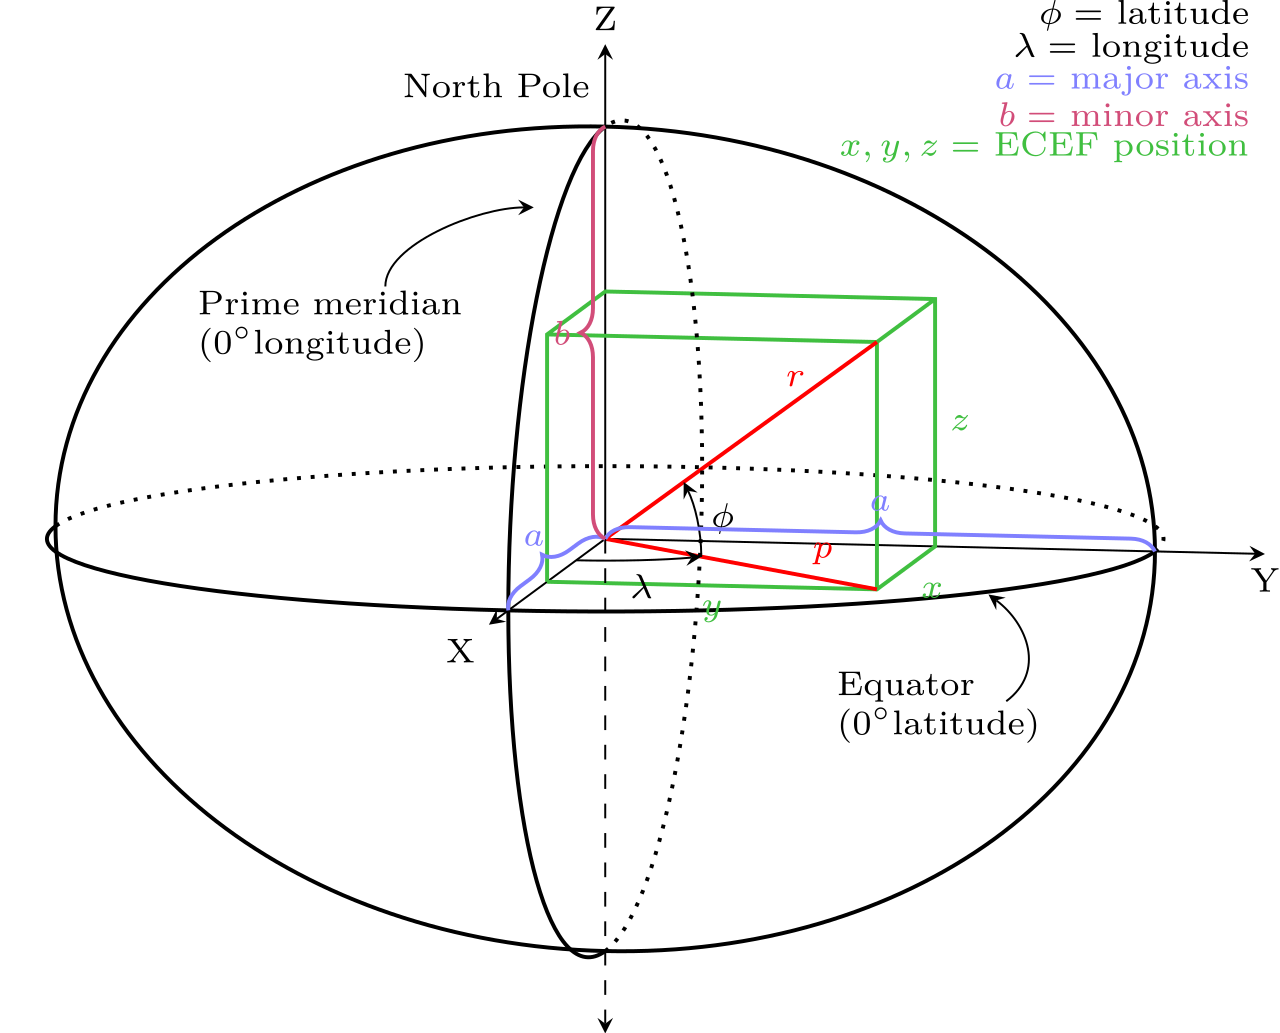
\includegraphics[width=0.60\textwidth]{FIG/ecef_wiki}
\caption{Zobrazení bodu v ECEF soustavě souřadnic. Obrázek je převzat z \cite{ecefWiki}.}
\label{fig:ecef}
\end{center}
\end{figure}

Základní kartézská pravouhlá soustava souřadníc, naúříklad tak, jako je zobrazená na obrázku \ref{fig:ecef}, je definována takto \cite{Soler1988}, \cite{Kovar2016}:

\begin{itemize}
\item počátek soustavy je soustředěn v geocentre, t.j. v gravitačním středu zemského tělesa,
\item osa \textbf{Z} směruje do místa zemského severního pólu, který je definován podle IERS. Protože poloha pólu sa v čase mění, používá se střední poloha zemského pólu (CTP).
\item osa \textbf{X} prochází bodem nulové zeměpisné délky, t.j. Greenwich poledníkem, který je definován podle IERS a míři do průsečníku tohto poledníku a roviny rovníku,
\item osa \textbf{Y} doplňuje pravotočivý pravouhlý sýstém souřadníc.
\end{itemize}

\subsubsection{ENU - East-North-Up}

Některé výpočty souřadníc je praktičtější provádět v lokální souřadnicové soustavě například vzdálenosť radarového přijímače od daného bodu atp.,\cite{Kovar2016}, \cite{Mayer2002}. ENU je lokální pravouhlá soustava souřadnic, pričemž její definice a umístnění počátku soustavy a souřadnicových os, dle značení na obrázku \ref{fig:enu}, jsou:
 
\begin{itemize}
\item počátek systému soustavy souřadníc je umiestnený v středě regiónu záujmu a to  buď na povrchu anebo blízko povrchu referenčního tělesa (elipsoid, koule),
\item osa \textbf{n} (North) směruje na sever, 
\item osa \textbf{e} (East) směruje na východ a 
\item osa \textbf{u} (Up) je totožná s normálou referenčního tělesa (elipsoid, koule). 
\end{itemize}

\begin{figure}[ht!]
\begin{center}

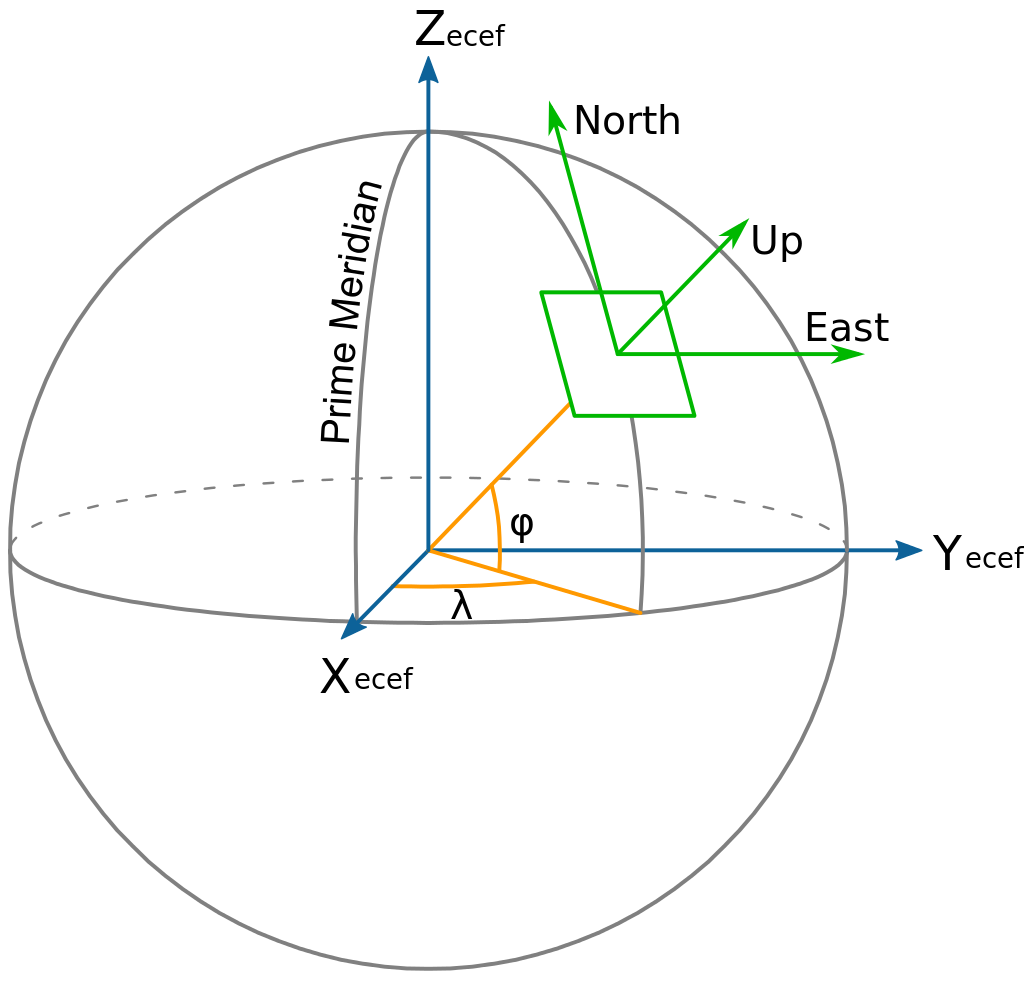
\includegraphics[width=0.50\textwidth]{FIG/enu_wiki}
\caption{Zobrazení systému souřadnic East-North-Up. Obrázek je převzat z \cite{enuWiki}.}
\label{fig:enu}
\end{center}
\end{figure}

\subsubsection{GEOD - Systém geodetických souřadníc}

\begin{figure}[ht!]
\begin{center}
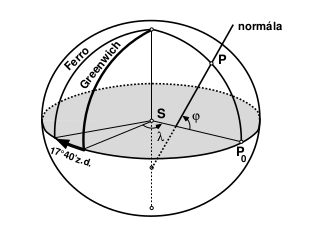
\includegraphics[width=0.50\textwidth]{FIG/geod_cimb}
\caption{Geodetické zeměpisné souřadnice. Obrázek je převzat z \cite{Cimbalnik1997}.}
\label{fig:geod}
\end{center}
\end{figure}

V praktických úlohách se poloha bodu popisuje pomocí geodetických anebo elipsoidických souřadníc. Elipsoidických proto, protože se definuje pomocí zvoleného zemského elipsoidu. Ten slouží k aproximaci fyzického zemského tělesa. Základní matematické vzorce určené pro odvození elipsoidu jsou obsahem přílohy \ref{appRefEll} a přehled konstant globálne užitých elipsoidů jsou obsahem přílohy \ref{appRefEllConst}.

Poloha bodu \textbf{P} na obrázku \ref{fig:geod} se vyjadřuje třemi souřadnicemi:

\begin{enumerate}
\item geodetickou zeměpisnou šířkou $\varphi$,
\item geodetickou zeměpisnou délkou $\lambda$,
\item geodetickou výškou.
\end{enumerate} 

Geodetická zeměpisná šířka $\varphi$ bodu \textbf{P} je uhel, který svírá normála v bodě P k povrchu elipsoidu, s rovinou rovníku. Geodetická zeměpisná délka $\lambda$ je úhel, který svírá rovina poledníku tohoto bodu s rovinou nultého poledníku. Za nultý poledník je mezinárodně volen ten, který prochází stabilizovaným bodem na astronomické observatoři v Greenwich. Geodetická výška se měří podél normály mezi referenčním elipsoidem a bodem \textbf{P}.

\subsubsection{SPHERE - Systém sférických súradníc}

Koule je základní a nejjednoduchší aproximace zemského tělesa. Sférické souřadnice tvoří systém souřdnic, které popisujou polohu bodu na sféře. Referenční koule je pak definovaná sférickým poloměrem. Pro praktické výpočty se jeho hodnota často zpočíta jako středný pomoměr křivosti (a to z důvodu zachování objemu eliposidu během jeho zobrazení na kouli, t.j. v místě lokálni aproximace - viz příloha \ref{appRefEll}).
 
\begin{figure}[ht!]
\begin{center}
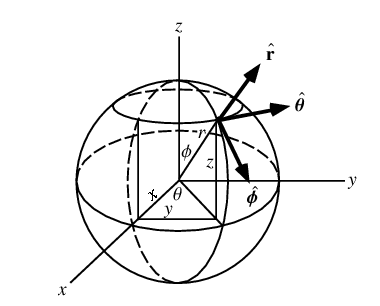
\includegraphics[width=0.50\textwidth]{FIG/sphere_wolf}
\caption{Sférické polárni souřadnice. Obrázek je převzat z \cite{sphereWolf}.}
\label{fig:sphere}
\end{center}
\end{figure}

Dle situace zobrazené na obrázku \ref{fig:sphere}, poloha bodu na sféře je vyjadřená soustavou tří souřadníc:
\begin{itemize}
\item $\theta$ hodnota azimutu v rovině rovníka. Pokud je uhel značený symbolem $\lambda$, pak poukazuje na zeměpisnou délku,
\item $\phi$ hodnota polárniho úhla počítaná od zenitu (také zenitový úhel). Pokud je uhel značený symbolem $\varphi^{'}$, pak poukazuje na doplnek zemepisej délky od zenitu, t.j. $\varphi = 90 - \varphi^{'}$ a
\item r, je středný polomer Zeme.
\end{itemize}

\newpage

\subsubsection{AES - Systém polárnych súradníc}

AES je súradný systém, ktorý pozostáva z týchto súradníc: azimut, elevačný uhol a spojnica medzi lokálnym počiatkom a cieľom. Jedná sa o systém polárnych súradníc. Lokálny počiatok súradného systému je charakterizovaný geodetickými súradnicami $lat_{0}, lon_{0}, h_{0}$. Na obrázku \ref{fig:aes} je tento systém názorne zobrazený.

\begin{figure}[ht!]
\begin{center}
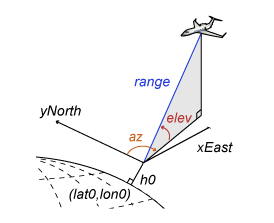
\includegraphics[width=0.50\textwidth]{FIG/AES}
\caption{Polární souřadnice. Obrázek je převzat z \cite{aesMatlab}.}
\label{fig:aes}
\end{center}
\end{figure}

